\documentclass[a4paper]{article}
\usepackage[margin=1.5cm]{geometry}

%\documentclass[11pt]{article}
%\usepackage[paperwidth=9cm,paperheight=60cm,margin=0.4cm]{geometry}

\usepackage{multicol}
\usepackage{enumitem}
\usepackage{graphicx}

%Links
\usepackage[colorlinks = true,
            linkcolor = blue,
            urlcolor  = blue,
            citecolor = blue,
            anchorcolor = blue]{hyperref}

%Simbolos matemáticos
\usepackage{amsmath}
\usepackage{amssymb}

%Enumeracion
\usepackage{enumitem}

%Páginas sin numeración
\pagestyle{empty}

%Interlineado
\renewcommand{\baselinestretch}{1.5}

%Arreglar comillas
\usepackage [autostyle]{csquotes}
\MakeOuterQuote{"}

%Macros
\newcommand{\Item}{\item[\stepcounter{enumii}$\blacktriangleright$\textbf{(\alph{enumii})}]} %Negrita en algunos items
\newcommand{\answer}{\item[**]}
\newcommand{\exercise}{\item}

%Logic macros
\newcommand{\then}{\to}
\newcommand{\eq}{\leftrightarrow}
\newcommand{\xor}{\veebar}
\newcommand{\nor}{\downarrow}
\newcommand{\nimply}{\nrightarrow}
\newcommand{\nand}{\uparrow}
\newcommand{\Then}{\Rightarrow}
\newcommand{\Eq}{\Leftrightarrow}


\begin{document}

\noindent \hrulefill 
\vspace{-7pt}
\begin{center} 
	\textbf{ Práctica 1: Lógica proposicional y de primer orden } \\
	Comisión: Rodrigo Cossio-Pérez y Leonardo Lattenero
\end{center}
\vspace{-10pt}
\hrulefill


\begin{enumerate}

	\exercise Demostrar que las siguientes relaciones son de equivalencia, indicar sus clases de equivalencia y el conjunto cociente.
	%\begin{multicols}{2}
	\begin{enumerate} [label=(\alph*)]
		\item La relación $ \sim = \left\lbrace (x,y) \in \mathbb{Z}^{2} ~|~ \exists k \in \mathbb{Z} ~~(x-y=2k) \right\rbrace$ donde $x \sim y$ se lee como "$x$ tiene la misma paridad que $y$".
		
		\item La relación $ \sim = \left\lbrace (x,y)\in \mathbb{Z}^{2} ~|~ x^{2}=y^{2} \right\rbrace$ donde $x \sim y$ se lee como "$x$ tiene el mismo cuadrado que $y$".
		
		\item Considerando un rectángulo $L_{1}$ de lados $a$ y $b$ con área $a.b$ y otro rectángulo $L_2$ de lados $c$ y $d$ con área $c.d$, donde $a,b,c,d \in ( 0 , +\infty)$. Se define la relación $ \sim = \left\lbrace (L_1,L_2) ~|~ a.b=c.d ~\right\rbrace$ donde $L_{1}\sim L_{2}$ se lee como "$L_{1}$ tiene la misma área que $L_{2}$".
		
		\item Considerando la fracción $q_1$ representada por $\displaystyle\frac{a}{b}$ y otra fracción $q_2$ representada por $\displaystyle\frac{c}{d}$, con $a,c\in\mathbb{Z}$ y $b,d\in\mathbb{Z}\setminus\{0\} $. Se define la relación: $\sim = \left\lbrace (q_1,q_2) ~|~ a.d=c.b \right\rbrace$ donde $q_{1}\sim q_{2}$ se lee como "$q_{1}$ es una fracción equivalente a $q_{2}$".
		\answer Reflexividad: $\forall a,b:  \left(\frac{a}{b}\right) R \left(\frac{a}{b}\right)$ ya que $a.b=a.b$. \\ Simetría: $\forall a,b,c,d: \left(\frac{a}{b}\right) R \left(\frac{c}{d}\right) \to \left(\frac{c}{d}\right) R \left(\frac{a}{b}\right)$ ya que $a.d=c.b \to c.b=a.d$. \\ Transitividad: $\forall a,b,c,d,e,f:  \left(\frac{a}{b}\right) R \left(\frac{c}{d}\right) \land \left(\frac{c}{d}\right) R \left(\frac{e}{f}\right) \to \left(\frac{a}{b}\right) R \left(\frac{e}{f}\right)$ \\ ya que $(a.d=c.b) \land (c.f=e.d) ~~\Then~~ (a.d=c.b) \land (c=\frac{e.d}{f}) ~~\Then~~ a.d=\frac{e.d}{f}.b ~~\Then~~ a=\frac{e}{f}.b ~~\Then~~ af=eb$

	\end{enumerate}
	%\end{multicols}


	\exercise Averiguar si las siguientes relaciones son de orden amplio u orden estricto y demostrarlo
	%\begin{multicols}{2}
	\begin{enumerate} [label=(\alph*)]
		\item Dada la relación $R$ definida en $\mathbb{R}$, se establece la relación como "$x$ es menor o igual que $y$" donde $x\mathrel{R}y$ se anota $x\leq y$ definida de la forma $R = \left\lbrace (x,y) ~|~ \exists k \in [0,+\infty) ~~( y=x+k ) \right\rbrace$
		\answer Relación de orden amplio (transitiva, antisimétrica, reflexiva) 

		\item Dada la relación $R$ definida en $\mathbb{R}$, se establece la relación como "$x$ es divisor de $y$" donde $x\mathrel{R}y$ se anota $x~|~y$ definida de la forma $R = \left\lbrace (x,y) ~|~ \exists n \in \mathbb{N} ~~( y=n.x ) \right\rbrace$
		\answer Relación de orden amplio (transitiva, antisimétrica, reflexiva)

		\item Dados dos conjuntos $A$ y $B$ se define la relación "$A$ es subconjunto de en $B$" donde $x\mathrel{R}y$ se anota $A\subseteq B$ definida de la forma $R = \left\lbrace (A,B) ~|~ \forall x \in A ~~( x\in A \to x\in B) \right\rbrace$
		\answer Relación de orden amplio (transitiva, antisimétrica, reflexiva)
		
		\item Dada la relación $R$ definida en $\mathbb{R}$, se establece la relación "$x$ es menor que $y$" donde $x\mathrel{R}y$ se anota $x<y$ definida de la forma $R = \left\lbrace (x,y) ~|~ \exists k \in (0,+\infty) ~~(y=x+k)  \right\rbrace$
		\answer Relación de orden estricto (transitiva, asimétrica e irreflexiva)
	\end{enumerate}
	%\end{multicols}


	\exercise Considerando el siguiente árbol genealógico: \\ \begin{center} 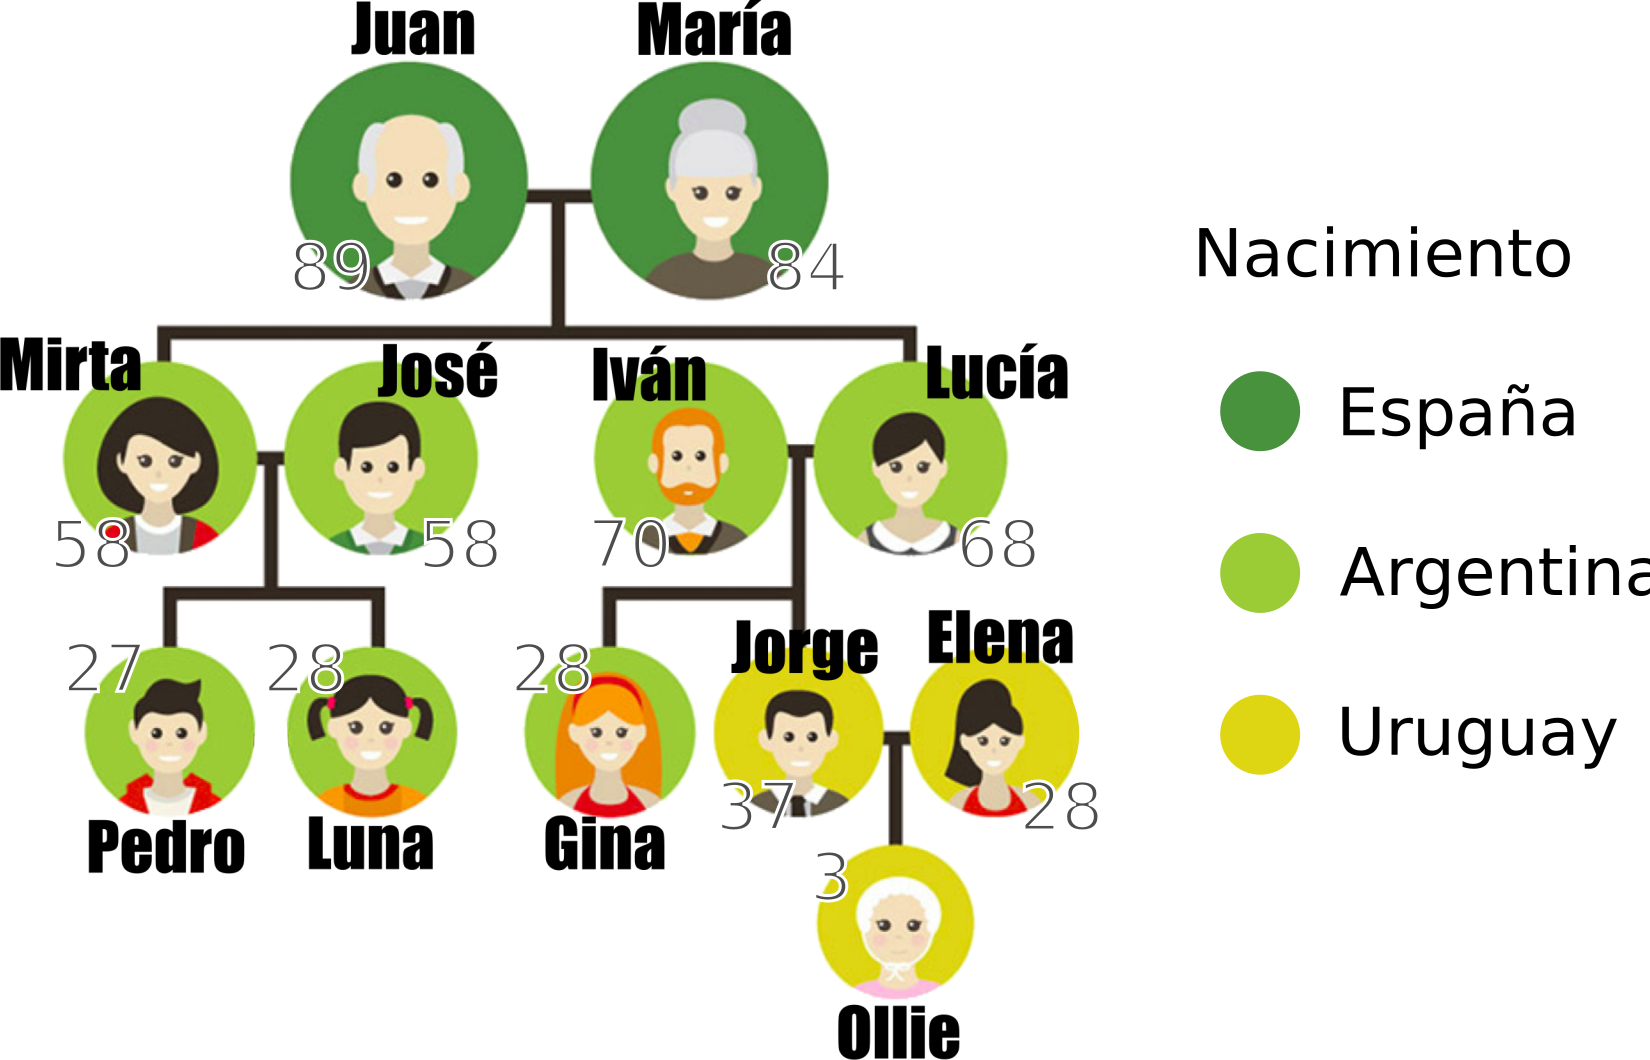
\includegraphics[height=5cm]{familia.png} \end{center}
	%\begin{multicols}{2}
	\begin{enumerate} [label=(\alph*)]
		\item Verificar que la relación "x tiene el mismo color de pelo que y" es una relación de equivalencia y representarla con un grafo. Indicar las clases de equivalencia y el conjunto cociente.

		\item Verificar que la relación "x nació en el mismo país que y" es una relación de equivalencia y representarla con un grafo. Indicar las clases de equivalencia y el conjunto cociente.
		
		\item Verificar que la relación "x es descendiente de y" es una relación de orden estricto parcial. Representar la relación en un diagrama de Hasse.
		
		\item Explicar porque la relación "x es de la misma edad o mayor que y" NO ES una relación de orden amplio.
		\answer Porque no es antisimétrica. (Mirta)$\mathrel{R}$(José) $\land$ (José)$\mathrel{R}$(Mirta) pero José$\neq$Mirta. También se puede verificar con Luna, Gina y Elena, que tienen la misma edad.
	
	\end{enumerate}
	%\end{multicols}

	\exercise Resolver los siguientes ejercicios variados
	%\begin{multicols}{2}
	\begin{enumerate} [label=(\alph*)]

		\item Sean $R_1$ y $R_2$ dos relaciones de equivalencia en $A$. Averiguar si $R_1 \cap R_2$ y $R_1 \cap R_2$ son relaciones de equivalencia en $A$.
		\answer $R_1 \cap R_2$ es de equivalencia mientras que no necesariamente lo es $R_1 \cap R_2$.

		\item Sea R una relación definida en el conjunto de número reales tal que $x R y$ si y solo si $x$ e $y$difieron por menos de 1, es decir, $|x-y|<1$. Demostrar que $R$ no es una relación de equivalencia.
		\answer $R$ es reflexiva porque $|x - x| = 0 < 1$. \\ $R$ es simétrica ya que $|x - y|=|y - x|$ por lo que $|x-y|<1 ~\Then~ |y - x| < 1$. \\ $R$ NO es transitiva. Contraejemplo: $x = 2.8$, $y = 1.9$, y $z = 1.1$, donde se ve que $|2.8-1.9|=0.9<1$, $|1.9-1.1|=0.8<1$, pero $|2.8-1.1|=1.7>1$. \\ Por lo tanto, $R$ no es una relación de equivalencia.

		\item En $\mathbb{Z}$ se define la relación $R$ mediante: $(a,b) \in R \Eq a^2+a=b^2+b$. Clasificar $R$.

		\item En $\mathbb{R}^2$ se define la relación $\sim$ mediante: $(x,y) \sim (x',y') \Eq y=y'$. Probar que $\sim$ es de equivalencia, determinar las clases de equivalencia y el conjunto cociente.

		\item En $A=\{1,2,4,6,8\}$ se define la siguiente relación: $xRy \Eq 3|x+y$. Definir $R$ por extensión, clasificarla y realizar su gráfico o esquema.

		\item En $\mathbb{N}^2$ se define la siguiente relación: $(a,b)=(a',b') \Eq a+b'=a'+b$. Demostrar que es de equivalencia, obtener las clases de equivalencia, el conjunto cociente y representarla indicando las clases.

		\item El conjunto $\{\{a\},\{b,c\},\{d\}\}$ es una partición de $A$. Obtener la relación de equivalencia asociada a la partición.

		\item En el conjunto $A=\{1,2,3,4,5\} \subseteq B$ se considera la relación de menor o igual. Determinr, si los hubiere, los elementos maximales y minimales, el conjunto de cotas superiores e inferiores, y el supremo e ínfimo.

		\item En \mathbb{R}, ordenado por la relación de menor o igual, se define el conjunto $A=\left\{ x \in \mathbb{R} ~|~ x=\frac{1}{n} \land n\in \mathbb{N} \right\}$. Averiguar si $A$ tiene primer y ultimo elemento, si es un conjunto bien ordenado, y en el caso de que admita cotas, si tiene supremo e ínfimo.

		\item Sea $R$ una relación definida en el conjunto de personas tal que $xRy$ si y solo si $x$ es mayor (en edad) que $y$. Averiguar si $R$ es una relación de orden amplio/estricto total/parcial.

	\end{enumerate}
	%\end{multicols}

	\exercise Obtener, si existen, el conjunto de cotas superiores e inferiores de los siguientes conjuntos y el supremo e ínfimo, considerando el superconjunto y la relación de orden dados.
	%\begin{multicols}{2}
	\begin{enumerate} [label=(\alph*)]
		\item $A=(0,1] \subseteq \mathbb{R}$ con la relación $\leq$ (menor o igual).
		\item $B=[-6,5] \subseteq \mathbb{R}$ con la relación $\leq$ (menor o igual).
		\item $C=(-6,5) \subseteq \mathbb{R}$ con la relación $\leq$ (menor o igual).
		\item $\mathcal{P}(A) \subseteq \mathcal{P}(B)$ con la relación $\subseteq$ (subconjunto de) con $A=\{1,2,3,4}$ y $B={1,2,3}$.
	\end{enumerate}
	%\end{multicols}

\end{enumerate}

\end{document}